\documentclass[9pt,pdftex,aspectratio=1610]{beamer}
\usepackage{amsmath, amsthm, amssymb}
\usepackage{color}
\usepackage{hyperref}
\usepackage{subfigure}
\usepackage{tabularx}
\usepackage{ragged2e}
\usepackage{booktabs}
\usepackage{multirow}
\usepackage{natbib}

\usecolortheme{dolphin}
\linespread{1.3}
\definecolor{nblue}{RGB}{0,0,128}

\bibliographystyle{ecta}
\setbeamercovered{transparent}

\newcolumntype{Y}{>{\RaggedRight\arraybackslash}X}
%\setbeamerfont{alerted text}{series=\bfseries}

\hypersetup{colorlinks=true, linkcolor=nblue,
citecolor=nblue, urlcolor=nblue, bookmarks=false,
pdfpagemode=UseNone,
pdfstartview={XYZ null null 1.25},
pdftitle={Heterogeneous Agent Trade},
pdfauthor={ Michael E. Waugh},
pdfkeywords={economics, trade, dynamics, quant econ, consumption, data science,
waugh, incomplete markets, inequality, Ricardo, julia, Armington, China, trade war, tariffs, python, matplotlib}}

%\usepackage[pdftex,colorlinks=true, bookmarks=false,
%pdfstartview={XYZ null null 1.0},
%pdftitle={Heterogeneous Agent Trade},
%pdfauthor={Michael E. Waugh},
%pdfkeywords={economics, trade, dynamics, quant econ, consumption, data science,
%waugh, incomplete markets, inequality, Ricardo, julia, Armington, China, trade war, tariffs, python, matplotlib},
%colorlinks=true,linkcolor=darkgray,citecolor=darkgray,urlcolor=darkgray,
%breaklinks]{hyperref}

\setbeamertemplate{navigation symbols}{}
\setbeamertemplate{footline}[frame number]
\setbeamertemplate{theorems}[numbered]
\setbeamertemplate{itemize subitem}[circle]
\setbeamertemplate{enumerate items}[default]

\setbeamerfont{frametitle}{size= \large}
\setbeamerfont{ framesubtitle }{size = \footnotesize}
\setbeamertemplate{frametitle}
{
\medskip
\smallskip
{\textsf{\underline{\insertframetitle\phantom{))))))))}}}}}
\setbeamertemplate{items}[circle]
\setbeamertemplate{itemize subitem}[circle]

\theoremstyle{definition}


\newtheorem{as}{Assumption}
\newtheorem{df}{Definition}
\newtheorem{lm}{Lemma}
\newtheorem{prp}{Proposition}

\usepackage[normalem]{ulem}
\newcommand\redout{\bgroup\markoverwith
{\textcolor{red}{\rule[.5ex]{1pt}{1pt}}}\ULon}

\makeatletter
\def\blfootnote{\xdef\@thefnmark{}\@footnotetext}
\makeatother

%%%%%%%%%%%%%%%%%%%%%%%%%%%%%%%%%%%%%%%%%%%%%%%%%%%%%%%%%%%%%%%%%%%%%%%%%%%%%%%%%%%%%%%%%%%%%%%%%
%%%%%%%%%%%%%%%%%%%%%%%%%%%%%%%%%%%%%%%%%%%%%%%%%%%%%%%%%%%%%%%%%%%%%%%%%%%%%%%%%%%%%%%%%%%%%%%%%

%%%%%%%%%%%%%%%%%%%%%%%%%%%%%%%%%%%%%%%%%%%%%%%%%%%%%%%%%%%%%%%%%%%%%%%%%%%%%%%%%%%%%%%%%%%%%%%%%
%%%%%%%%%%%%%%%%%%%%%%%%%%%%%%%%%%%%%%%%%%%%%%%%%%%%%%%%%%%%%%%%%%%%%%%%%%%%%%%%%%%%%%%%%%%%%%%%%

\title{\Large Heterogeneous Agent Trade}
\institute[Foo and Bar]{\normalsize\begin{tabular}[h]{c}
Michael E. Waugh  \\
Federal Reserve Bank of Minneapolis\blfootnote{The views expressed herein are those of the author and not necessarily those of the Federal
Reserve Bank of Minneapolis or the Federal Reserve System. This project was developed with research support from the National Science Foundation (NSF Award number 1948800). Thomas Hasenzagl provided excellent research assistance.} and NBER\\
\href{https://twitter.com/tradewartracker}{@tradewartracker}
\end{tabular}}

\date{\today}

\begin{document}

\begin{frame}
\titlepage
\setcounter{framenumber}{0}
\section{}
\end{frame}

\begin{frame}[t]{What am I doing?}
\smallskip
Big picture | these are the questions that interest me\ldots\\
\smallskip
\textbf{1.} What are distributional consequences of trade?\\
\smallskip
\textbf{2.} Is there a role for trade policy to improve outcomes?\\
\bigskip
One mechanism behind \textbf{1.} is heterogeneity in expenditure shares on traded goods and \begin{alert}{\textbf{elasticities}}\end{alert}.
\begin{itemize}
\smallskip
\item \citet*{auer2022unequal} is a nice example. In the context of the 2015 Swiss appreciation, they find that poor households are more price elastic.
\end{itemize}
\bigskip
\medskip
This paper:\\
\smallskip
GE, heterogenous agent model of trade delivering ABLV-like facts. I work out the implications for
aggregate trade, the gains from trade, and the normative implications for trade policy.
\end{frame}

%%%%%%%%%%%%%%%%%%%%%%%%%%%%%%%%%%%%%%%%%%%%%%%%%%%%%%%%%%%%%%%%%%%%%%%%%%%%%%%%%%%%%%%%%%%%%%%%%
%%%%%%%%%%%%%%%%%%%%%%%%%%%%%%%%%%%%%%%%%%%%%%%%%%%%%%%%%%%%%%%%%%%%%%%%%%%%%%%%%%%%%%%%%%%%%%%%%

\begin{frame}[t]{How I do it\ldots}
\smallskip
Two ingredients:
\begin{itemize}
\smallskip
\item Standard incomplete markets model with households facing incomplete insurance against idiosyncratic productivity and taste shocks.
\smallskip
\item Trade as in Armington (national varieties), but households have random utility over these varieties.
\end{itemize}
\bigskip
Qualitatively I characterize\ldots
\begin{itemize}
\smallskip
\item How price elasticities vary at the micro-level and how (and if) micro-heterogeneity shapes aggregate trade and trade elasticities.
\smallskip
\item The welfare gains from trade at the micro and macro level.
\smallskip
\item The efficient allocation and, thus, how market incompleteness shapes these outcomes.
\end{itemize}
\bigskip
Quantitatively, I compute the a 19 country model (the \citet{eaton2002technology} data) and (today) study the welfare gains to small reductions in trade costs.
\end{frame}

%%%%%%%%%%%%%%%%%%%%%%%%%%%%%%%%%%%%%%%%%%%%%%%%%%%%%%%%%%%%%%%%%%%%%%%%%%%%%%%%%%%%%%%%%%%%%%%%%
%%%%%%%%%%%%%%%%%%%%%%%%%%%%%%%%%%%%%%%%%%%%%%%%%%%%%%%%%%%%%%%%%%%%%%%%%%%%%%%%%%%%%%%%%%%%%%%%%

\begin{frame}[t]{Model: Production and Trade}
\smallskip
$M$ countries. Each country produces a nationally differentiated product as in Armington.\\
\bigskip
\medskip
In country $i$, competitive firms' produce variety $i$ with:
\begin{align*}
Q_i = A_i N_i,
\end{align*}
where $A_i$ is TFP; $N_i$ are efficiency units of labor supplied by households.\\
\bigskip
\medskip
Cross-country trade faces obstacles:
\begin{itemize}
\smallskip
\item iceberg trade costs $d_{ij} > 1$ for one unit from supplier $j$ to go to buyer $i$.
\end{itemize}
\bigskip
\medskip
This structure leads to the following prices that households face
\begin{align*}
p_{ij} = \frac{d_{ij}w_{j}}{A_{j}}.
\end{align*}
\end{frame}

%%%%%%%%%%%%%%%%%%%%%%%%%%%%%%%%%%%%%%%%%%%%%%%%%%%%%%%%%%%%%%%%%%%%%%%%%%%%%%%%%%%%%%%%%%%%%%%%%
%%%%%%%%%%%%%%%%%%%%%%%%%%%%%%%%%%%%%%%%%%%%%%%%%%%%%%%%%%%%%%%%%%%%%%%%%%%%%%%%%%%%%%%%%%%%%%%%%

\begin{frame}[t]{Model: Households I}
\smallskip
Mass of $L_i$ households in each country $i$.\\
\medskip
Household-level preferences:
\begin{align*}
\small
&  \mathrm{E}\sum_{t = 0}^{\infty} \beta^{t} \ \tilde{u}( \{ c_{ijt}, \epsilon_{jt} \}_{M})\\
\\
& \mbox{where}  \ \ \  \tilde{u}( c_{ijt}, \epsilon_{jt} ) =  u(c_{ijt}) + \epsilon_{jt}.
\end{align*}
\begin{itemize}
\item $\epsilon_{jt}$ is iid (across time and households) taste shocks over national varieties.
\end{itemize}
\medskip
Assumptions:
\begin{itemize}
\smallskip
\item For most of the analysis, I'll only assume $u$ is well behaved.
\smallskip
\item $\epsilon_{jt}$s are distributed Type 1 Extreme Value with dispersion parameter $\sigma_{\epsilon}$.
\end{itemize}
\end{frame}

%%%%%%%%%%%%%%%%%%%%%%%%%%%%%%%%%%%%%%%%%%%%%%%%%%%%%%%%%%%%%%%%%%%%%%%%%%%%%%%%%%%%%%%%%%%%%%%%%
%%%%%%%%%%%%%%%%%%%%%%%%%%%%%%%%%%%%%%%%%%%%%%%%%%%%%%%%%%%%%%%%%%%%%%%%%%%%%%%%%%%%%%%%%%%%%%%%%

\begin{frame}[t]{Model: Households II}
\smallskip
A household's efficiency units $z_t$ evolve according to a Markov Chain. They face the wage per efficiency unit $w_{it}$.\\
\bigskip
\medskip
Households borrow or accumulate a non-state contingent asset, $a$, with gross return $R_{i}$. Household's face the debt limit
\begin{align*}
a_{t+1} \geq - \phi_{i}
\end{align*}\\
\bigskip
\medskip
Conditional on a variety choice, a household's budget constraint is
\begin{align*}
p_{ij}c_{ijt} +  a_{t+1} \leq    R_{i} a_{t} + w_{it} z_{t}.
\end{align*}
\end{frame}

%%%%%%%%%%%%%%%%%%%%%%%%%%%%%%%%%%%%%%%%%%%%%%%%%%%%%%%%%%%%%%%%%%%%%%%%%%%%%%%%%%%%%%%%%%%%%%%%%
%%%%%%%%%%%%%%%%%%%%%%%%%%%%%%%%%%%%%%%%%%%%%%%%%%%%%%%%%%%%%%%%%%%%%%%%%%%%%%%%%%%%%%%%%%%%%%%%%

\begin{frame}[t]{What Households Do\ldots}
\smallskip
Focus on a stationary setting. A hh's state are its asset holdings $a$ and shock $z$.\\
\bigskip
\uncover<2->{\textbf{1.} The hh makes a variety choice (e.g. a US or Italian variety) and how much to consume. The choice probability is:
\begin{align*}
\pi_{ij}(a, z) = \exp \left( \frac{ v_{ij}(a, z) }{\sigma_{\epsilon}} \right) \Bigg / \sum_{j'} \exp \left( \frac{ v_{ij'}(a, z) }{\sigma_{\epsilon}} \right),
\end{align*}
where $v_{ij}(a, z)$ is the hh's value function conditional on a choice.}\\
\bigskip
\medskip
\uncover<3->{\textbf{2.} The hh makes an asset choice. Away from the constraint, asset choices (conditional on a variety choice) must respect this Euler Equation:
\begin{align*}
\frac{u'(c_{ij}(a,z))}{p_{ij}} = \beta \mathrm{E}_{z'} \bigg \{ -\sigma_{\epsilon} \frac{\partial \pi_{ii}(a',z') / \pi_{ii}(a',z')}{\partial a'} + \frac{u'(c_{ii}(a',z'))R_i}{p_{ii}} \bigg \},
\end{align*}
where I'm exploiting an ACR-like feature that ex-ante value functions can be expressed in terms of $i,i$ home choices.}
\end{frame}
%%%%%%%%%%%%%%%%%%%%%%%%%%%%%%%%%%%%%%%%%%%%%%%%%%%%%%%%%%%%%%%%%%%%%%%%%%%%%%%%%%%%%%%%%%%%%%%%%
%%%%%%%%%%%%%%%%%%%%%%%%%%%%%%%%%%%%%%%%%%%%%%%%%%%%%%%%%%%%%%%%%%%%%%%%%%%%%%%%%%%%%%%%%%%%%%%%%


\begin{frame}[t]{Aggregation}
\smallskip
Aggregates arise from explicit aggregation of hh-level actions. Two examples:\\
\bigskip
\medskip
Aggregate, bilateral imports and exports are
\begin{align*}
M_{ij} = L_i \int_{z} \int_{a}  p_{ij} c_{ij}(a, z) \pi_{ij}(a, z) \lambda_i(a, z), \ \ \ \ \ X_{ji} = L_j \int_{z} \int_{a}  p_{ji} c_{ji}(a, z) \pi_{ji}(a, z) \lambda_i(a, z),
\end{align*}
where $\lambda_i$ is the distribution of hhs across states and $c_{ij}(a, z)$ is the consumption function. Here trade flows take on a mixed logit formulation as in \citet*{berry1995automobile}. \\
\bigskip
\medskip
The national income accounting identity (GDP = C + I + G + X - M) \ldots
\begin{align*}
p_{i} Y_{i}  =  \underbrace{L_{i} \sum_{j} \int_{z} \int_{a}  p_{ij} c_{ij}(a, z) \pi_{ij}(a, z) \lambda_i(a, z)}_{\widetilde{P_{i} C_i}} \ + \ \underbrace{\bigg[\ \sum_{j\neq i}X_{ji} -  \sum_{j\neq i}M_{ij} \bigg]}_{-R_{i}A_i + A_{i}'}.
\end{align*}
Notice how trade is non-trivially connected to a county's capital account.
\end{frame}

%%%%%%%%%%%%%%%%%%%%%%%%%%%%%%%%%%%%%%%%%%%%%%%%%%%%%%%%%%%%%%%%%%%%%%%%%%%%%%%%%%%%%%%%%%%%%%%%%
%%%%%%%%%%%%%%%%%%%%%%%%%%%%%%%%%%%%%%%%%%%%%%%%%%%%%%%%%%%%%%%%%%%%%%%%%%%%%%%%%%%%%%%%%%%%%%%%%
\begin{frame}[t]{Equilibrium}
\smallskip
\textbf{The Decentralized Stationary Equilibrium.} A Decentralized Stationary Equilibrium are asset policy functions and commodity choice probabilities $\{\  g_{ij}(a, z), \pi_{ij}(a, z) \ \}_{ij}$, probability distributions $\{ \ \lambda_i(a, z) \ \}_{i}$ and positive real numbers $\left \{w_i, p_{ij}, R_i\right \}_{ij}$ such that
\begin{itemize}
\smallskip
\item[i]  Prices ($w_i, p_{ij}$) satisfy the firms problem;
\item[ii] The policy functions and choice probabilities solve the household's optimization problem;
\item[iv] The probability distribution $\lambda_i(a, z)$ induced by the policy functions, choice probabilities, and primitives satisfies the law of motion and is stationary;
\item[v] Goods market clears:
\begin{align*}
p_{i} Y_{i} - \sum_{j}^{M}  X_{ji} = 0, \ \ \forall i
\end{align*}
\item[v] Bond market clears with
\begin{align*}
\mathrm{A_i'} = 0, \ \ \forall i.
\end{align*}
\end{itemize}
\end{frame}

%%%%%%%%%%%%%%%%%%%%%%%%%%%%%%%%%%%%%%%%%%%%%%%%%%%%%%%%%%%%%%%%%%%%%%%%%%%%%%%%%%%%%%%%%%%%%%%%
%%%%%%%%%%%%%%%%%%%%%%%%%%%%%%%%%%%%%%%%%%%%%%%%%%%%%%%%%%%%%%%%%%%%%%%%%%%%%%%%%%%%%%%%%%%%%%%%


\begin{frame}[t]{The H-A Trade Elasticity}
\smallskip
\textbf{Proposition \#1: The H-A Trade Elasticity.} The trade elasticity between country $i$ and country $j$ is:
\begin{align}
\theta_{ij} = 1 + \int_{a} \int_{z} \bigg \{ \theta_{ij}(a,z)^{I} + \theta_{ij}(a,z)^{E} \bigg \}\omega_{ij}(a,z) - \bigg \{ \theta_{ii}(a,z)^{I} + \theta_{ii}(a,z)^{E} \bigg \}\omega_{ii}(a,z), \nonumber
\end{align}
which is the difference between $ij$ and $ii$ expenditure-weighted micro-level elasticities. The micro-level elasticities for households with states $a,z$ are an intensive and extensive elasticity
\begin{align}
\nonumber
\begin{alert}<2>{\theta_{ij}(a,z)^{I} = \frac{\partial c_{ij}(a,z)/ c_{ij}(a,z)}{\partial d_{ij} / d_{ij}}}\end{alert}, \ \ \ \ \ \ \begin{alert}<3>{\theta_{ij}(a,z)^{E} = \frac{\partial \pi_{ij}(a,z) / \pi_{ij}(a,z)}{\partial d_{ij} / d_{ij}}}\end{alert}, \ \ \ \
\end{align}
and $\omega_{ij}(a,z)$ are the expenditure weights.\\
\only<2>{
\medskip
{\small \begin{align*}
\begin{alert}<2>{\theta_{ij}(a,z)^{I} = \bigg [-\frac{\partial g_{ij}(a,z)/ p_{ij}c_{ij}(a,z)}{\partial p_{ij}/ p_{ij}} - 1 \bigg ]\frac{\partial p_{ij}/p_{ij}}{\partial d_{ij}/ d_{ij}}.}\end{alert}
\end{align*}}\\
\medskip
The idea here is that reduction in trade costs relaxes the hh's budget constraint and then the division of new resources between assets and expenditure determines the intensive margin elasticity.}
\only<3>{
\medskip
{\small
\begin{align*}
\begin{alert}<3>{\theta_{ij}(a,z)^{E}}\end{alert} = - \frac{\partial \Phi_{i}(a,z) / \Phi_{i}(a,z)}{\partial d_{ij}/d_{ij}} + \begin{alert}<3>{\frac{1}{\sigma_{\epsilon}}\frac{\partial v_{ij}(a,z)}{\partial d_{ij}/d_{ij}} }\end{alert}.
\end{align*}}\\
Key is \begin{alert}<3>{$\frac{\partial v_{ij}(a,z)}{\partial d_{ij}/d_{ij}}$}\end{alert}.\\
\bigskip
In the paper, I show that if relative risk aversion $ > 1$ than hh's with (i) high $u'(c)$ and (ii) high MPCs are more price elastic. \begin{alert}<3>{\textbf{So poor hh's are the most price sensitive.}}\end{alert}}
\end{frame}

%%%%%%%%%%%%%%%%%%%%%%%%%%%%%%%%%%%%%%%%%%%%%%%%%%%%%%%%%%%%%%%%%%%%%%%%%%%%%%%%%%%%%%%%%%%%%%%%
%%%%%%%%%%%%%%%%%%%%%%%%%%%%%%%%%%%%%%%%%%%%%%%%%%%%%%%%%%%%%%%%%%%%%%%%%%%%%%%%%%%%%%%%%%%%%%%%


\begin{frame}[t]{Trade Elasticities by HH-Level State}
\vspace{-.5cm}
\begin{figure}[t]
\centerline{
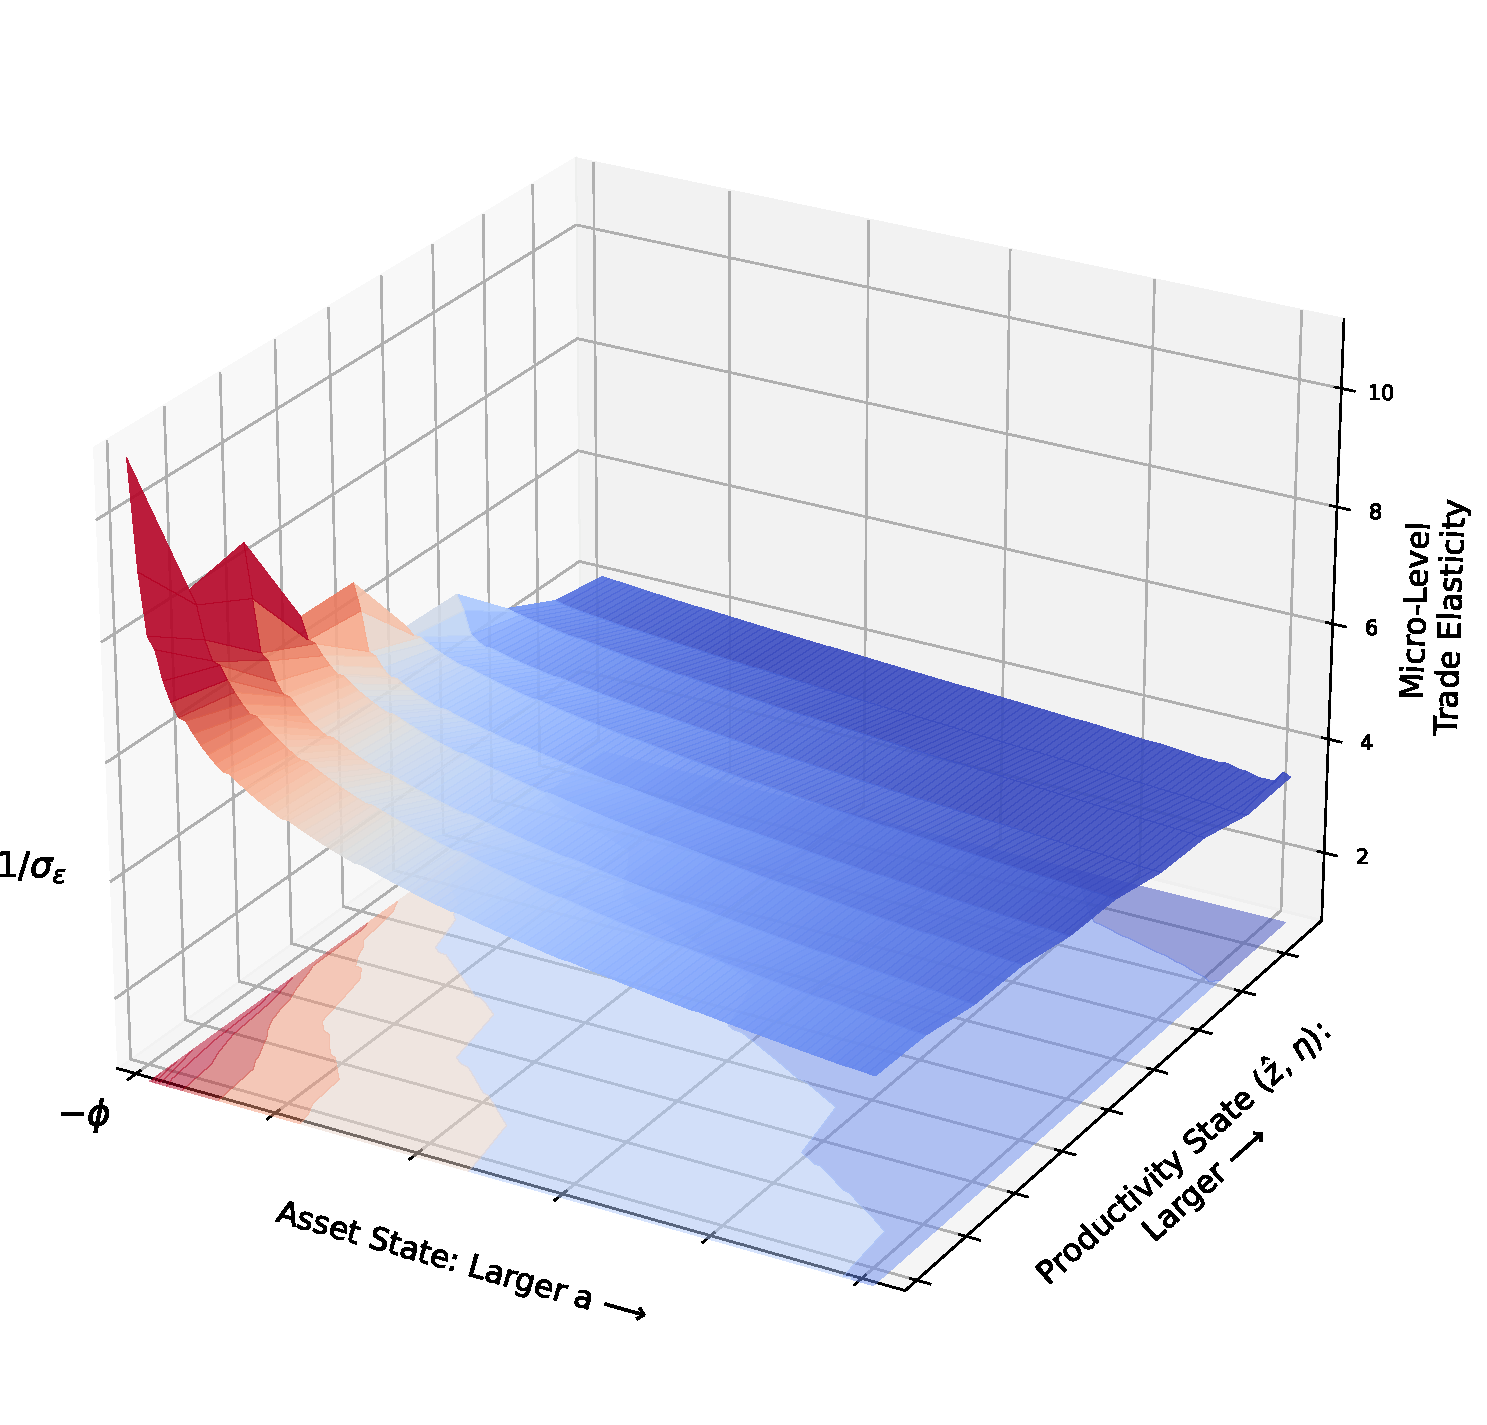
\includegraphics[scale = 0.5]{../notes/figures/micro-elasticity.pdf}}
\end{figure}
\end{frame}


\begin{frame}[t]{Trade Shares: $M_{ij}(a,z) / M_{ii}(a,z)$, by HH-Level State}
\vspace{-.5cm}
\begin{figure}[t]
\centerline{
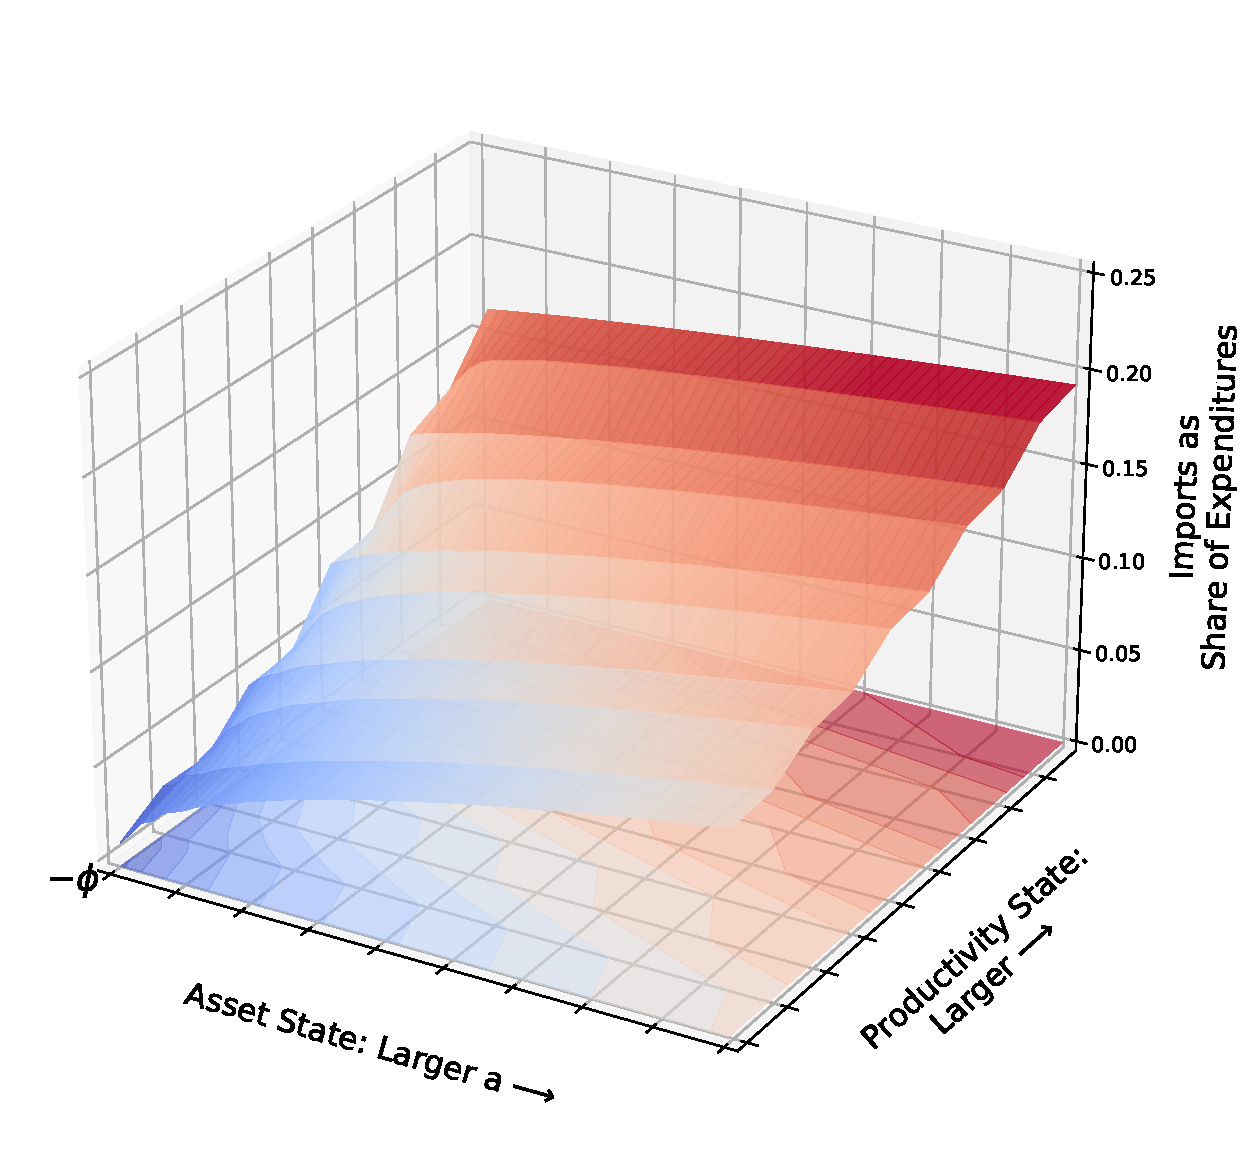
\includegraphics[scale = 0.5]{../notes/figures/trade-share.pdf}}
\end{figure}
\end{frame}


\begin{frame}[t]{H-A Gains from Trade}
\smallskip
\textbf{Proposition \#2: H-A Welfare Gains from Trade.} The gains from trade under a utilitarian social welfare function are
\begin{align*}
\frac{\mathrm{d} W_{i}}{\mathrm{d} d_{ij} / d_{ij}} = \int_{z} \int_{a}  \bigg \{ \underbrace{\frac{\mathrm{d} v_i(a, z)}{\mathrm{d} d_{ij} / d_{ij}}}_{\small \mbox{gains to hh}}  + \underbrace{v_{i}(a,z) \frac{\mathrm{d} \lambda_{i}(a,z)/ \lambda_{i}(a,z)}{\mathrm{d} d_{ij} / d_{ij}}}_{\small \mbox{gains to reallocation}}   \bigg \} L_i \lambda_{i}(a,z),
\nonumber
\end{align*}
where $v_i$ is a hh's value function before taste shocks are realized.\\
\medskip
Household-level gains are
\begin{align*}
\frac{\mathrm{d} v_i(a, z)}{\mathrm{d} d_{ij} / d_{ij}} = \mathbb{E}_{z} \sum_{t = 0}^{\infty} \beta^{t} \bigg \{ -\sigma_{\epsilon} \frac{\mathrm{d} \pi_{ii}(a_{t},z_{t}) / \pi_{ii}(a_{t},z_{t})}{\mathrm{d}d_{ij} / d_{ij}} + u'(c_{ii}(a_{t},z_{t}))a_{t} \frac{\mathrm{d} R_{i}}{\mathrm{d} d_{ij} / d_{ij}} \bigg \}.
\end{align*}\\
\bigskip
\medskip
HH-level gains pick up two effects:
\begin{itemize}
\item An ACR-like term reflecting how it's home choice changes\ldots basically the gains from substitution.
\smallskip
\item How the value of a hh's wealth changes through GE effects on interest rates.
\end{itemize}
\end{frame}

%%%%%%%%%%%%%%%%%%%%%%%%%%%%%%%%%%%%%%%%%%%%%%%%%%%%%%%%%%%%%%%%%%%%%%%%%%%%%%%%%%%%%%%%%%%%%%%%
%%%%%%%%%%%%%%%%%%%%%%%%%%%%%%%%%%%%%%%%%%%%%%%%%%%%%%%%%%%%%%%%%%%%%%%%%%%%%%%%%%%%%%%%%%%%%%%%

\begin{frame}[t]{H-A Gains from Trade: $\log$ Preferences $\Rightarrow$ Separation of Trade and Heterogeneity}
\smallskip
\textbf{Proposition \#3: Separation of Trade and Micro-Heterogeneity.} In the dynamic, heterogenous agent trade model where preferences are logarithmic over the physical commodity
\begin{align}
\tilde{u}( c_{ijt}, \epsilon_{jt} ) =  \log(c_{ij,t}) + \epsilon_{j,t}, \nonumber
\end{align}
the trade elasticity is
\begin{align}
\theta = -\frac{1}{\sigma_{\epsilon}}, \nonumber
\end{align}
and is independent of household heterogeneity. And the welfare gains from trade are
\begin{align}
\frac{\mathrm{d} W_{i}}{\mathrm{d} d_{ij} / d_{ij}} = -\frac{1}{\theta (1-\beta)} \times \frac{\mathrm{d} \pi_{ii} / \pi_{ii}}{\mathrm{d}d_{ij} / d_{ij}}. \nonumber
\end{align}
and is (i) independent of the household heterogeneity and (ii) summarized by the trade elasticity and the change in the home choice probability (and home share).\\
\bigskip
\medskip
Mimics the results of \citet{anderson1987ces} and \citet{arkolakis2012new}, remarkable as this is a far more complex economy\ldots
\end{frame}

%%%%%%%%%%%%%%%%%%%%%%%%%%%%%%%%%%%%%%%%%%%%%%%%%%%%%%%%%%%%%%%%%%%%%%%%%%%%%%%%%%%%%%%%%%%%%%%%
%%%%%%%%%%%%%%%%%%%%%%%%%%%%%%%%%%%%%%%%%%%%%%%%%%%%%%%%%%%%%%%%%%%%%%%%%%%%%%%%%%%%%%%%%%%%%%%%

\begin{frame}[t]{H-A Gains from Trade under Efficiency}
\smallskip
\textbf{Proposition \#4: Trade Elasticities and Welfare Gains in the Efficient Allocation} The trade elasticity between $i,j$ in the efficient allocation is:
\begin{align}
\theta_{ij} =  -\frac{1}{\sigma_{\epsilon}} \bigg [ u'(c_{ij}) c_{ij} \bigg]. \nonumber
\end{align}\\
\bigskip
And the welfare gains from a reduction in trade costs between $i,j$ are
\begin{align}
\frac{\mathrm{d} W}{\mathrm{d} d_{ij} / d_{ij}} = \frac{\partial W}{\partial d_{ij} / d_{ij}} = \frac{1}{1-\beta} \times u'(c_{ij}) c_{ij} \pi_{ij} L_i, \nonumber
\end{align}
which is the discounted, direct effect from relaxing the resource constraint.\\
\bigskip
\medskip
Mimics the results of \citet{AtkesonBurstein2010} but with household (not firm) heterogeneity.
\end{frame}

%%%%%%%%%%%%%%%%%%%%%%%%%%%%%%%%%%%%%%%%%%%%%%%%%%%%%%%%%%%%%%%%%%%%%%%%%%%%%%%%%%%%%%%%%%%%%%%%
%%%%%%%%%%%%%%%%%%%%%%%%%%%%%%%%%%%%%%%%%%%%%%%%%%%%%%%%%%%%%%%%%%%%%%%%%%%%%%%%%%%%%%%%%%%%%%%%

\begin{frame}[t]{Quantitative Analysis}
\smallskip
Preliminary. This is what I'm going to do:
\begin{itemize}
  \item Grab trade costs and productivity estimates from 19 country world of \citet{eaton2002technology} and compute an equilibrium.
\smallskip
  \item Explore small, global reduction in trade costs. No transition path today, ran out of time!
\end{itemize}
\bigskip
Other important parameters and how I set them for today.
\begin{itemize}
\item Taste shock parameter so $1 / \sigma_{\epsilon} = 4.0$. CRRA for $u$ with relative risk aversion $= 1.5$.
\smallskip
\item Earnings process is a mixture of a persistent and transitory component and calibrated as in\\ \citet*{krueger2016macroeconomics}.
\smallskip
\item Borrowing constraint is set $\approx 2\times$ earnings for US. Discount factor set so $R \approx$ 2\% for US.
\end{itemize}
\bigskip
My RA Thomas Hasenzagl and I have Julia and Python code to compute things pretty fast.
\end{frame}
%%%%%%%%%%%%%%%%%%%%%%%%%%%%%%%%%%%%%%%%%%%%%%%%%%%%%%%%%%%%%%%%%%%%%%%%%%%%%%%%%%%%%%%%%%%%%%%%
%%%%%%%%%%%%%%%%%%%%%%%%%%%%%%%%%%%%%%%%%%%%%%%%%%%%%%%%%%%%%%%%%%%%%%%%%%%%%%%%%%%%%%%%%%%%%%%%

\begin{frame}[t]{Bilateral Trade: Model vs. Data}
\begin{figure}[!t]
\centering{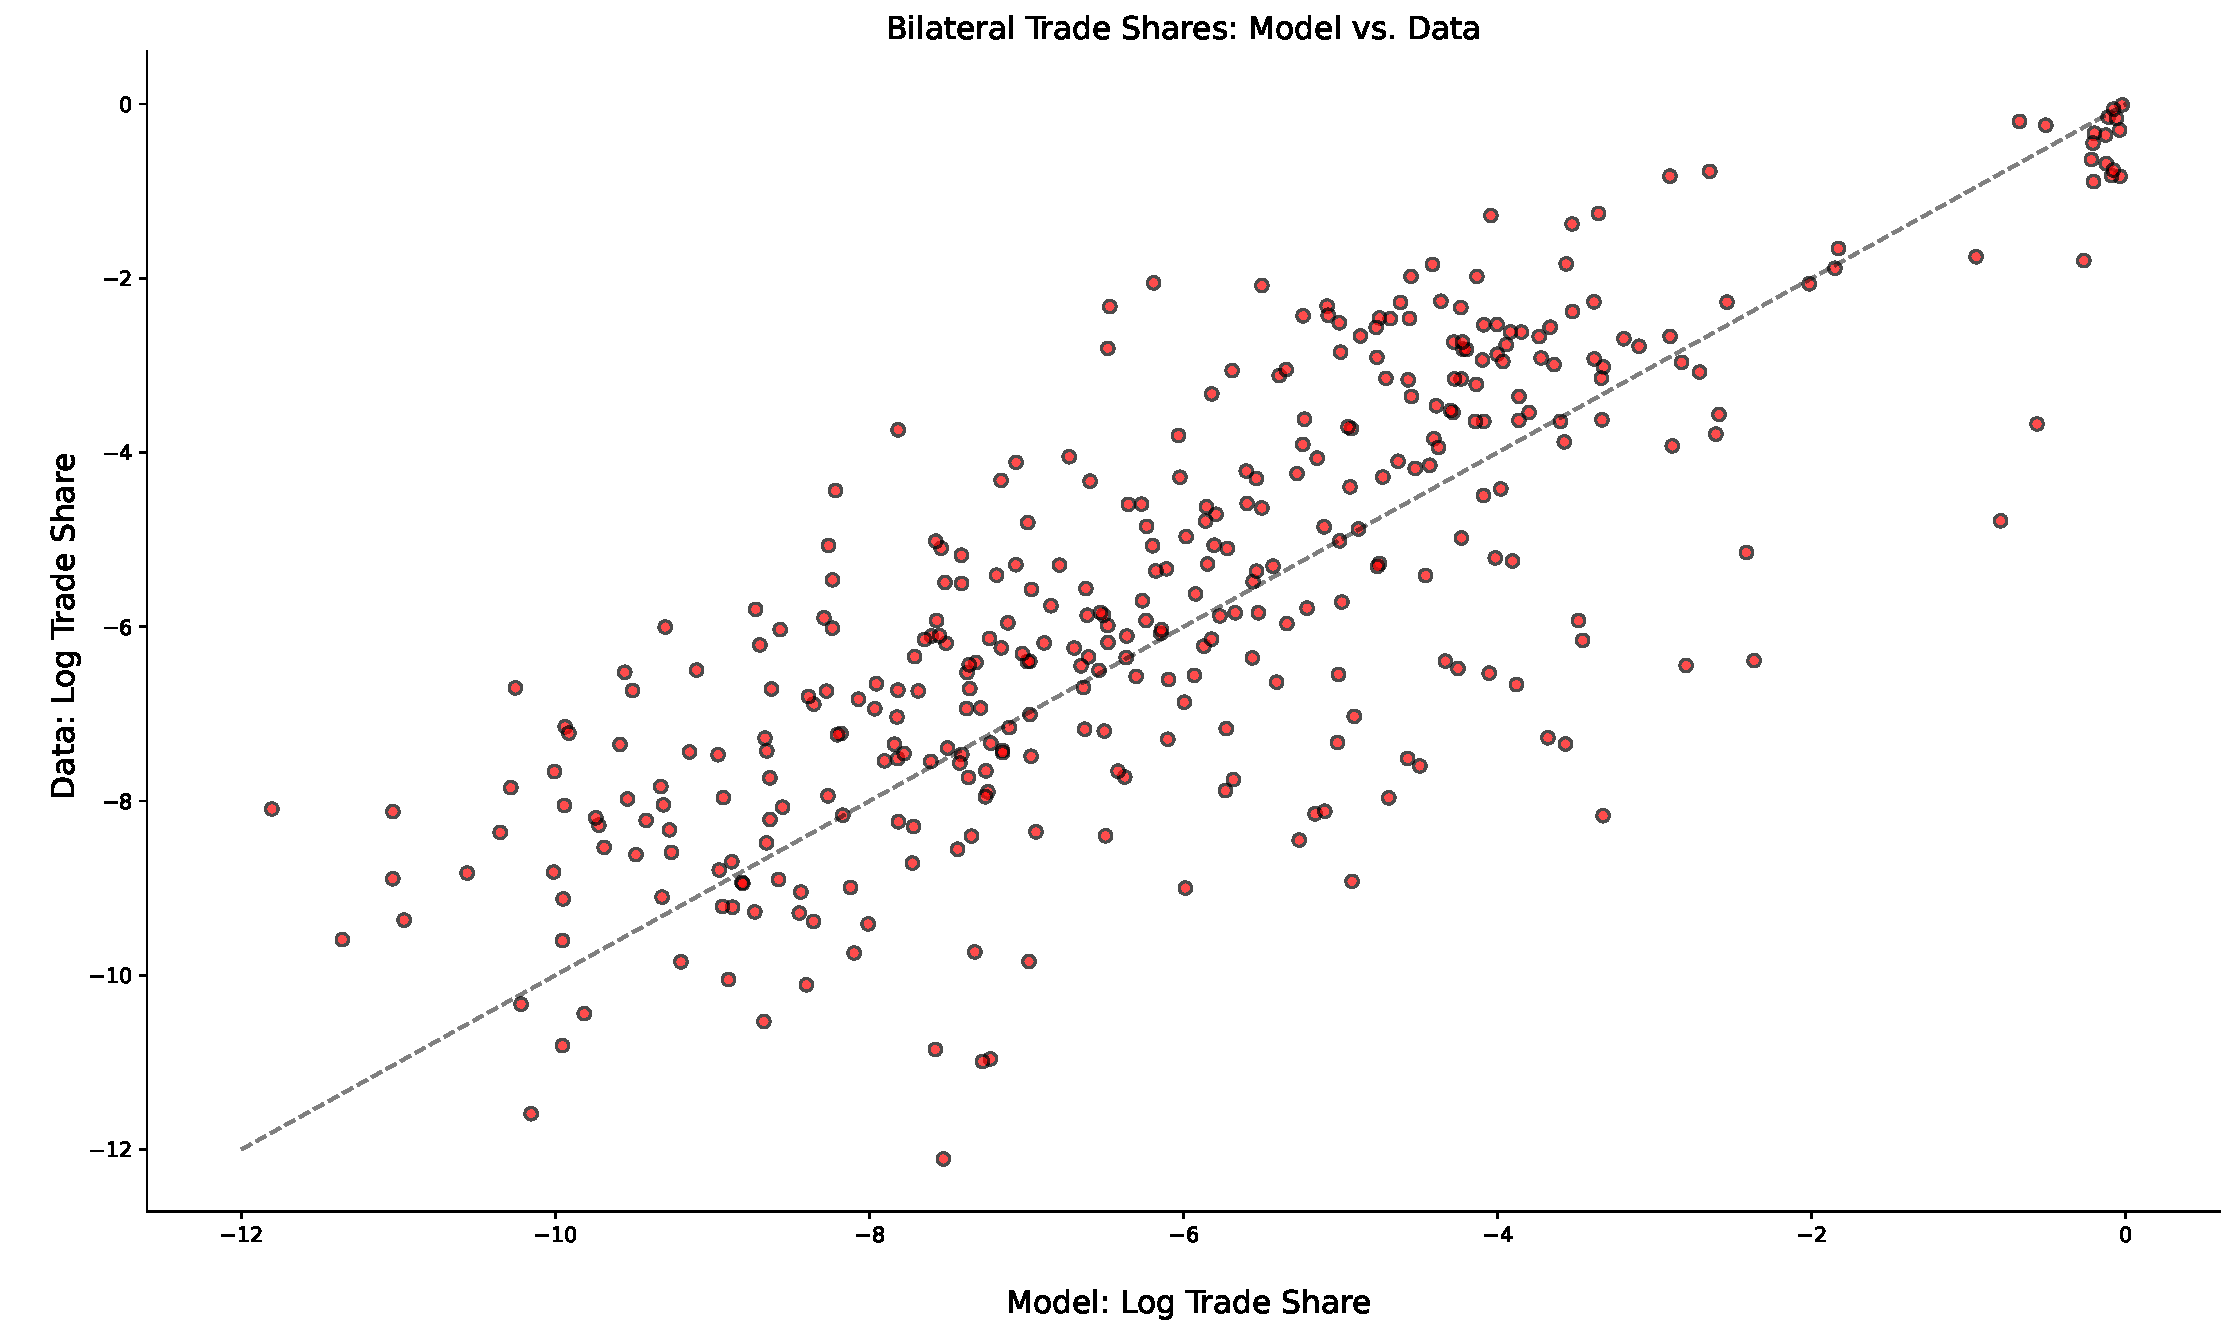
\includegraphics[scale = .35]{../notes/figures/trade-fit.pdf}}
\end{figure}
\end{frame}

%%%%%%%%%%%%%%%%%%%%%%%%%%%%%%%%%%%%%%%%%%%%%%%%%%%%%%%%%%%%%%%%%%%%%%%%%%%%%%%%%%%%%%%%%%%%%%%%
%%%%%%%%%%%%%%%%%%%%%%%%%%%%%%%%%%%%%%%%%%%%%%%%%%%%%%%%%%%%%%%%%%%%%%%%%%%%%%%%%%%%%%%%%%%%%%%%

\begin{frame}[t]
\frametitle{U.S. Welfare Gains to a Global 1\% Reduction in Trade Costs}
\begin{table}[t]
\footnotesize
\setlength {\tabcolsep}{6.05mm}
\renewcommand{\arraystretch}{1.80}
\begin{center}
\begin{tabular}{l c c c}
\multicolumn{4}{c}{\small \textbf{Trade and Welfare by Income --- Global {\color{red} 1\%} Reduction}}\\
\hline
\hline
& \footnotesize  Baseline & \multicolumn{2}{c}{1\% reduction} \\
\cmidrule(lr){2-2}  \cmidrule(lr){3-4}
\footnotesize  Income Quartile & \footnotesize  $1 - \pi_{ii}$ &  \footnotesize  $1 - \pi_{ii}$  & Welfare (\% Change) \\
\hline
\footnotesize  Bottom quartile  & 0.0179 & 0.0182 & 0.0006 \\
\footnotesize  Median & 0.0509 & 0.0515 & 0.0061 \\
\footnotesize  Upper quartile  & 0.0960 & 0.0972  & 0.0137\\
\footnotesize  Aggregate & 0.0744 & 0.0753  & 0.0078\\
\cmidrule(lr){2-2}  \cmidrule(lr){3-4}
\footnotesize  Interest rate & 2.14 & \multicolumn{2}{c}{2.15} \\
\footnotesize  \% losers & --- & \multicolumn{2}{c}{17.9}\\
\hline
\end{tabular}
%\parbox[c]{3.65in}{\vspace{.1cm}
%{\footnotesize \textbf{Note:}}}
\end{center}
\end{table}
\end{frame}



%%%%%%%%%%%%%%%%%%%%%%%%%%%%%%%%%%%%%%%%%%%%%%%%%%%%%%%%%%%%%%%%%%%%%%%%%%%%%%%%%%%%%%%%%%%%%%%%
%%%%%%%%%%%%%%%%%%%%%%%%%%%%%%%%%%%%%%%%%%%%%%%%%%%%%%%%%%%%%%%%%%%%%%%%%%%%%%%%%%%%%%%%%%%%%%%%

\begin{frame}[t]
\frametitle{U.S. Welfare Gains to a Global {\color{red} 10\%} Reduction in Trade Costs}
\begin{table}[t]
\footnotesize
\setlength {\tabcolsep}{6.05mm}
\renewcommand{\arraystretch}{1.80}
\begin{center}
\begin{tabular}{l c c c}
\multicolumn{4}{c}{\small \textbf{Trade and Welfare by Income --- Global {\color{red} 10\%} Reduction}}\\
\hline
\hline
& \footnotesize  Baseline & \multicolumn{2}{c}{1\% reduction} \\
\cmidrule(lr){2-2}  \cmidrule(lr){3-4}
\footnotesize  Income Quartile & \footnotesize  $1 - \pi_{ii}$ &  \footnotesize  $1 - \pi_{ii}$  & Welfare (\% Change) \\
\hline
\footnotesize  Bottom quartile  & 0.0179 & 0.0208 & 0.1247 \\
\footnotesize  Median & 0.0509 & 0.0583 & 0.1988 \\
\footnotesize  Upper quartile  & 0.0960 & 0.1094  & 0.2963\\
\footnotesize  Aggregate & 0.0744 & 0.0848  & 0.2185\\
\cmidrule(lr){2-2}  \cmidrule(lr){3-4}
\footnotesize  Interest rate & 2.14 & \multicolumn{2}{c}{2.17} \\
\footnotesize  \% losers & --- & \multicolumn{2}{c}{0.0}\\
\hline
\end{tabular}
%\parbox[c]{3.65in}{\vspace{.1cm}
%{\footnotesize \textbf{Note:}}}
\end{center}
\end{table}
\end{frame}

%%%%%%%%%%%%%%%%%%%%%%%%%%%%%%%%%%%%%%%%%%%%%%%%%%%%%%%%%%%%%%%%%%%%%%%%%%%%%%%%%%%%%%%%%%%%%%%%
%%%%%%%%%%%%%%%%%%%%%%%%%%%%%%%%%%%%%%%%%%%%%%%%%%%%%%%%%%%%%%%%%%%%%%%%%%%%%%%%%%%%%%%%%%%%%%%%

\begin{frame}[t]{U.S. Welfare Gains to a Global 1\% Reduction in Trade Costs}
\vspace{-.5cm}
\begin{figure}[!t]
\centering{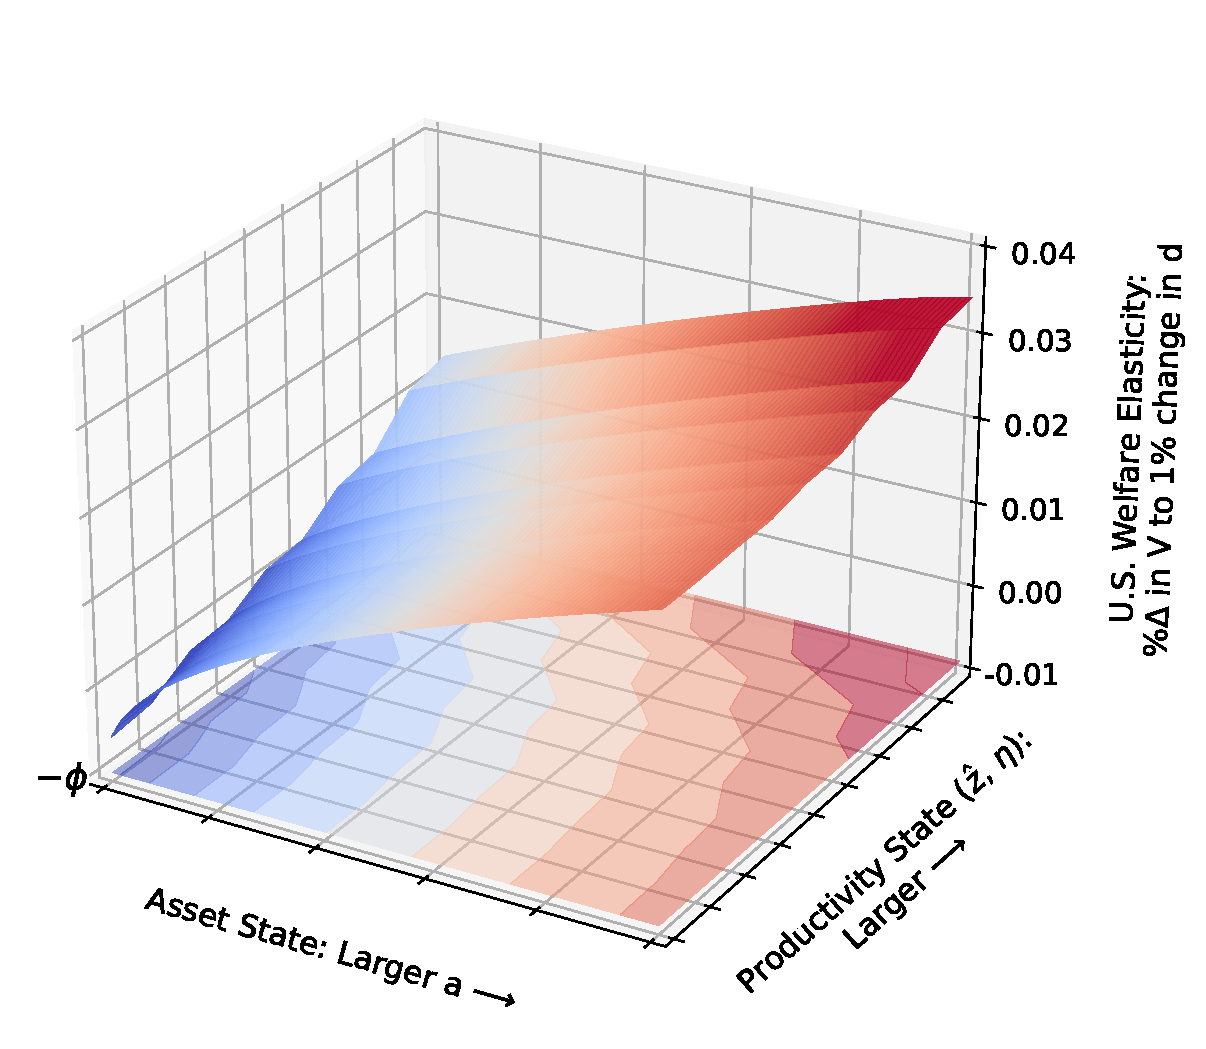
\includegraphics[scale = .5]{../notes/figures/welfare-elasticity.pdf}}
\end{figure}
\end{frame}


%%%%%%%%%%%%%%%%%%%%%%%%%%%%%%%%%%%%%%%%%%%%%%%%%%%%%%%%%%%%%%%%%%%%%%%%%%%%%%%%%%%%%%%%%%%%%%%%
%%%%%%%%%%%%%%%%%%%%%%%%%%%%%%%%%%%%%%%%%%%%%%%%%%%%%%%%%%%%%%%%%%%%%%%%%%%%%%%%%%%%%%%%%%%%%%%%

\begin{frame}[t]{Welfare Gains to a Global 1\% Reduction in Trade Costs}
\begin{table}[t]
\footnotesize
\setlength {\tabcolsep}{4.15mm}
\renewcommand{\arraystretch}{1.9}
\begin{center}
\begin{tabular}{l c c}
\multicolumn{3}{c}{\small \textbf{Welfare Gains to a Global 1\% Reduction in Trade Costs}}\\
\hline
\hline
\footnotesize   & \footnotesize  Baseline Model &  \footnotesize  Rep. Agent Model\\
\hline
\footnotesize  USA  & $\begin{array}{c}0.0075 \vspace{-.45cm}\\ \scriptstyle [ \ 83 \ ]\end{array}$   & $\begin{array}{c}0.025 \vspace{-.45cm}\\ \scriptstyle [ \ -- \ ]\end{array}$\\
\footnotesize  Germany  & $\begin{array}{c}0.14 \vspace{-.45cm}\\ \scriptstyle [ \ 100 \ ]\end{array}$   & $\begin{array}{c}0.31 \vspace{-.45cm}\\ \scriptstyle [ \ -- \ ]\end{array}$\\
\footnotesize  Japan  & $\begin{array}{c}0.004 \vspace{-.45cm}\\ \scriptstyle [ \ 80 \ ]\end{array}$   & $\begin{array}{c}0.014 \vspace{-.45cm}\\ \scriptstyle [ \ -- \ ]\end{array}$\\
\footnotesize  Canada  & $\begin{array}{c}0.09 \vspace{-.45cm}\\ \scriptstyle [ \ 100 \ ]\end{array}$   & $\begin{array}{c}0.18 \vspace{-.45cm}\\ \scriptstyle [ \ -- \ ]\end{array}$\\
\hline
\end{tabular}
\parbox[c]{3.1in}{\vspace{.1cm}
{\footnotesize \textbf{Note:} Numbers in brackets are \% of population who gain. Rep. Agent Model uses ACR calculation with trade elasticity $=$ 4.0}}
\end{center}
\end{table}
\end{frame}





%%%%%%%%%%%%%%%%%%%%%%%%%%%%%%%%%%%%%%%%%%%%%%%%%%%%%%%%%%%%%%%%%%%%%%%%%%%%%%%%%%%%%%%%%%%%%%%%
%%%%%%%%%%%%%%%%%%%%%%%%%%%%%%%%%%%%%%%%%%%%%%%%%%%%%%%%%%%%%%%%%%%%%%%%%%%%%%%%%%%%%%%%%%%%%%%%


\begin{frame}[t]
\frametitle{Where I'm headed next\ldots}
\smallskip
Lot's to do, but ``big picture'' this is where I'm aiming:\\
\bigskip
\textbf{1.} Can trade policy improve outcomes?
\begin{itemize}
\smallskip
\item This is a useful laboratory to think about policy because (i) there is scope for it and (ii) have a direct representation of utility (not an indirect representation).
\end{itemize}
\bigskip
\textbf{2.} How financial globalization relates globalization in goods trade?
\begin{itemize}
\smallskip
\item The model provides a coherent account of both trade in goods and assets. I think it'd be interesting to see what happens.
\end{itemize}
\end{frame}



%%%%%%%%%%%%%%%%%%%%%%%%%%%%%%%%%%%%%%%%%%%%%%%%%%%%%%%%%%%%%%%%%%%%%%%%%%%%%%%%%%%%%%%%%%%%%%%%
%%%%%%%%%%%%%%%%%%%%%%%%%%%%%%%%%%%%%%%%%%%%%%%%%%%%%%%%%%%%%%%%%%%%%%%%%%%%%%%%%%%%%%%%%%%%%%%%

\appendix

\newcounter{finalframe}
\setcounter{finalframe}{\value{framenumber}}

\begin{frame}[allowframebreaks]
\frametitle{References}
\scriptsize
\bibliography{../notes/bibtex/micro_price_bibtex}
\end{frame}


%%%%%%%%%%%%%%%%%%%%%%%%%%%%%%%%%%%%%%%%%%%%%%%%%%%%%%%%%%%%%%%%%%%%%%%%%%%%%%%%%%%%%%%%%%%%%%%%%
%%%%%%%%%%%%%%%%%%%%%%%%%%%%%%%%%%%%%%%%%%%%%%%%%%%%%%%%%%%%%%%%%%%%%%%%%%%%%%%%%%%%%%%%%%%%%%%%%

%%%%%%%%%%%%%%%%%%%%%%%%%%%%%%%%%%%%%%%%%%%%%%%%%%%%%%%%%%%%%%%%%%%%%%%%%%%%%%%%%%%%%%%%%%%%%%%%
%%%%%%%%%%%%%%%%%%%%%%%%%%%%%%%%%%%%%%%%%%%%%%%%%%%%%%%%%%%%%%%%%%%%%%%%%%%%%%%%%%%%%%%%%%%%%%%%

\begin{frame}[t]{Bilateral Trade Elasticities: German Example}
\begin{figure}[!t]
\centering{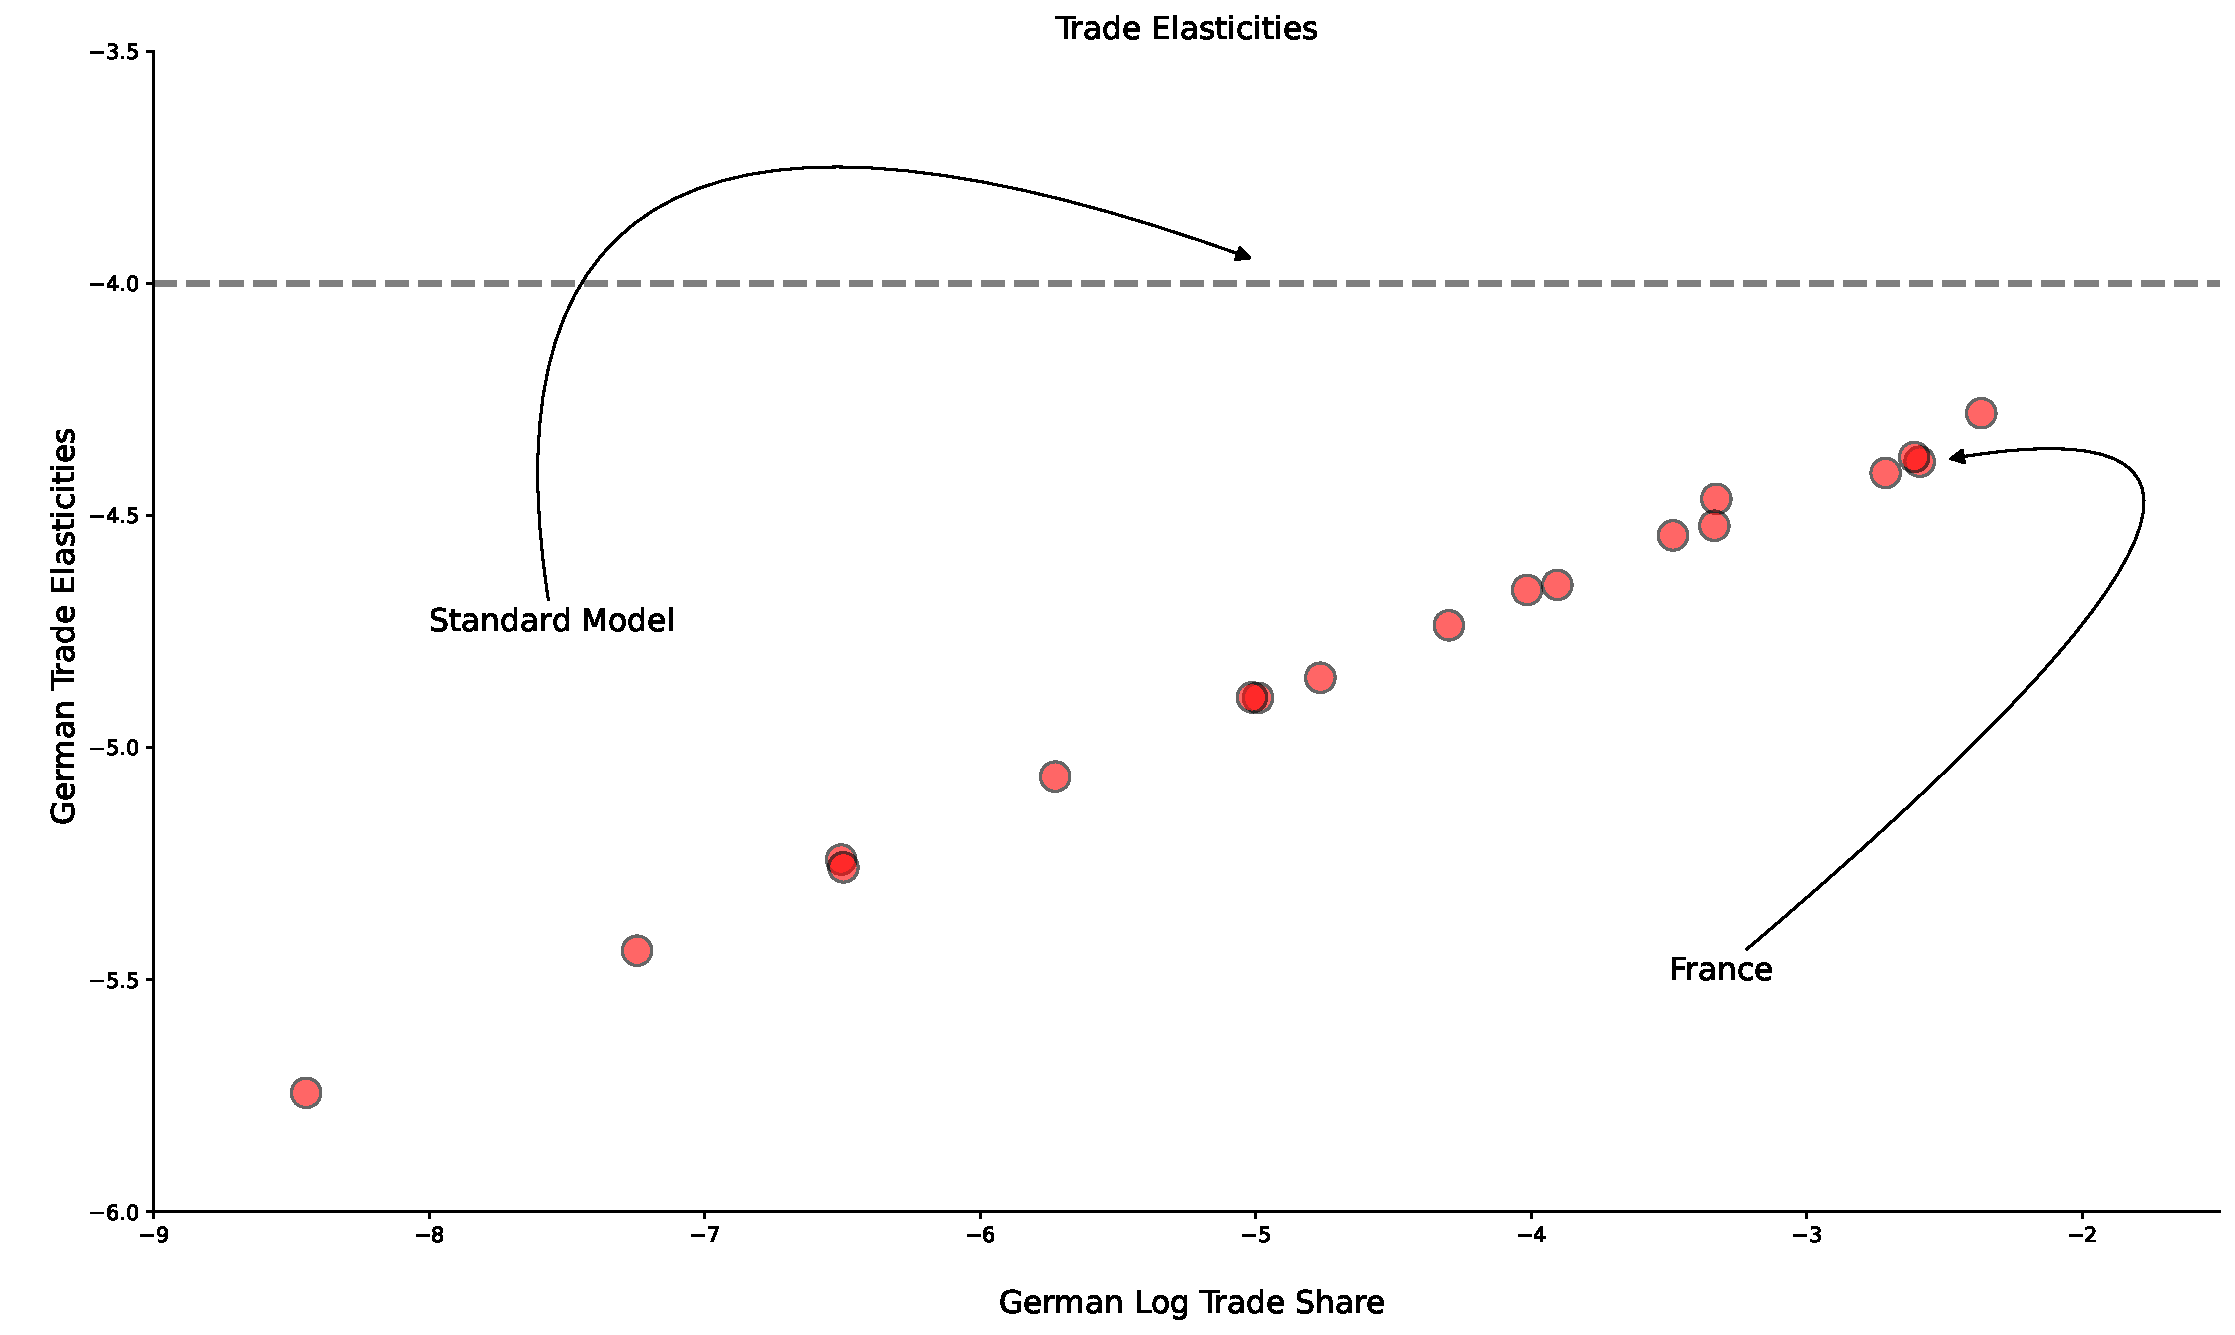
\includegraphics[scale = .35]{../notes/figures/german-trade-elasticities.pdf}}
\end{figure}
\end{frame}

%%%%%%%%%%%%%%%%%%%%%%%%%%%%%%%%%%%%%%%%%%%%%%%%%%%%%%%%%%%%%%%%%%%%%%%%%%%%%%%%%%%%%%%%%%%%%%%%
%%%%%%%%%%%%%%%%%%%%%%%%%%%%%%%%%%%%%%%%%%%%%%%%%%%%%%%%%%%%%%%%%%%%%%%%%%%%%%%%%%%%%%%%%%%%%%%%

\begin{frame}[t]{Welfare Gains to a Global \begin{alert}{10\%}\end{alert} Reduction in Trade Costs}
\begin{table}[t]
\footnotesize
\setlength {\tabcolsep}{4.15mm}
\renewcommand{\arraystretch}{1.9}
\begin{center}
\begin{tabular}{l c c}
\multicolumn{3}{c}{\small \textbf{Welfare Gains to a Global \begin{alert}{10\%}\end{alert} Reduction in Trade Costs}}\\
\hline
\hline
\footnotesize   & \footnotesize  Baseline Model &  \footnotesize  Rep. Agent Model\\
\hline
\footnotesize  USA  & $\begin{array}{c}0.21 \vspace{-.45cm}\\ \scriptstyle [ \ 100 \ ]\end{array}$   & $\begin{array}{c}0.28 \vspace{-.45cm}\\ \scriptstyle [ \ -- \ ]\end{array}$\\
\footnotesize  Germany  & $\begin{array}{c}1.6 \vspace{-.45cm}\\ \scriptstyle [ \ 100 \ ]\end{array}$   & $\begin{array}{c}3.5 \vspace{-.45cm}\\ \scriptstyle [ \ -- \ ]\end{array}$\\
\footnotesize  Japan  & $\begin{array}{c}0.14 \vspace{-.45cm}\\ \scriptstyle [ \ 100 \ ]\end{array}$   & $\begin{array}{c}0.21 \vspace{-.45cm}\\ \scriptstyle [ \ -- \ ]\end{array}$\\
\footnotesize  Canada  & $\begin{array}{c}1.13 \vspace{-.45cm}\\ \scriptstyle [ \ 100 \ ]\end{array}$   & $\begin{array}{c}1.9 \vspace{-.45cm}\\ \scriptstyle [ \ -- \ ]\end{array}$\\
\hline
\end{tabular}
\parbox[c]{3.1in}{\vspace{.1cm}
{\footnotesize \textbf{Note:} Numbers in brackets are \% of population who gains. Rep. Agent Model uses ACR calculation with trade elasticity $=$ 4.0}}
\end{center}
\end{table}
\end{frame}





\setcounter{framenumber}{\value{finalframe}}

%%%%%%%%%%%%%%%%%%%%%%%%%%%%%%%%%%%%%%%%%%%%%%%%%%%%%%%%%%%%%%%%%%%%%%%%%%%%%%%%%%%%%%%%%%%%%%%%%
%%%%%%%%%%%%%%%%%%%%%%%%%%%%%%%%%%%%%%%%%%%%%%%%%%%%%%%%%%%%%%%%%%%%%%%%%%%%%%%%%%%%%%%%%%%%%%%%%



\end{document} 